

\tikzset{every picture/.style={line width=0.75pt}} %set default line width to 0.75pt

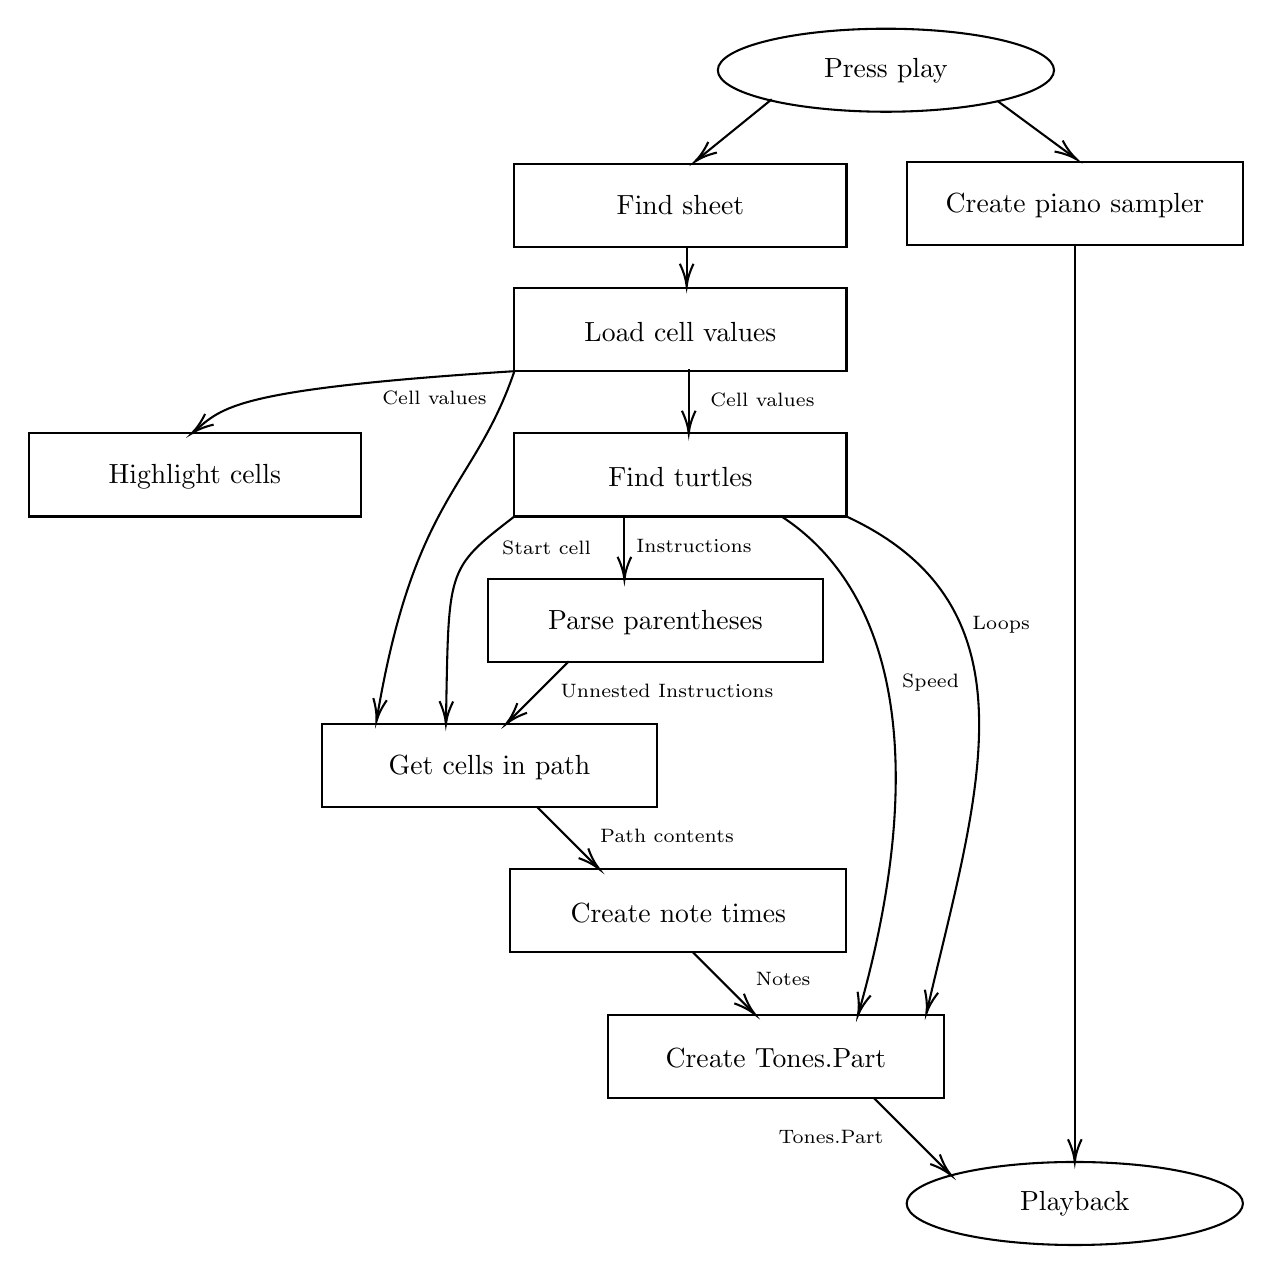
\begin{tikzpicture}[x=0.75pt,y=0.75pt,yscale=-1,xscale=1]
%uncomment if require: \path (0,604); %set diagram left start at 0, and has height of 604

%Shape: Rectangle [id:dp3390223975782729]
\draw   (244.5,71) -- (404.5,71) -- (404.5,111) -- (244.5,111) -- cycle ;

%Shape: Rectangle [id:dp7168559924493858]
\draw   (244.5,131) -- (404.5,131) -- (404.5,171) -- (244.5,171) -- cycle ;

%Shape: Rectangle [id:dp8835932361497658]
\draw   (433.7,70) -- (595.5,70) -- (595.5,110) -- (433.7,110) -- cycle ;

%Shape: Rectangle [id:dp9464422191216635]
\draw   (244.5,201) -- (404.5,201) -- (404.5,241) -- (244.5,241) -- cycle ;

%Shape: Rectangle [id:dp6384624480751633]
\draw   (231.6,271) -- (393.4,271) -- (393.4,311) -- (231.6,311) -- cycle ;

%Shape: Rectangle [id:dp2927464084046889]
\draw   (151.6,341) -- (313.4,341) -- (313.4,381) -- (151.6,381) -- cycle ;

%Shape: Rectangle [id:dp9052659554068596]
\draw   (242.6,411) -- (404.4,411) -- (404.4,451) -- (242.6,451) -- cycle ;

%Shape: Rectangle [id:dp5637329489183025]
\draw   (289.6,481) -- (451.4,481) -- (451.4,521) -- (289.6,521) -- cycle ;

%Curve Lines [id:da3917180624639185]
\draw    (244.5,241) .. controls (211.17,266.67) and (212.98,265.81) .. (211.52,339.88) ;
\draw [shift={(211.5,341)}, rotate = 271.14] [color={rgb, 255:red, 0; green, 0; blue, 0 }  ][line width=0.75]    (10.93,-3.29) .. controls (6.95,-1.4) and (3.31,-0.3) .. (0,0) .. controls (3.31,0.3) and (6.95,1.4) .. (10.93,3.29)   ;

%Straight Lines [id:da6961662223442007]
\draw    (297.5,241) -- (297.5,269.4) ;
\draw [shift={(297.5,271.4)}, rotate = 270] [color={rgb, 255:red, 0; green, 0; blue, 0 }  ][line width=0.75]    (10.93,-3.29) .. controls (6.95,-1.4) and (3.31,-0.3) .. (0,0) .. controls (3.31,0.3) and (6.95,1.4) .. (10.93,3.29)   ;

%Curve Lines [id:da9168950950169605]
\draw    (372.6,240.6) .. controls (431.31,278.41) and (442.88,365.52) .. (410.49,479.68) ;
\draw [shift={(410,481.4)}, rotate = 286.01] [color={rgb, 255:red, 0; green, 0; blue, 0 }  ][line width=0.75]    (10.93,-3.29) .. controls (6.95,-1.4) and (3.31,-0.3) .. (0,0) .. controls (3.31,0.3) and (6.95,1.4) .. (10.93,3.29)   ;

%Curve Lines [id:da7972588626438504]
\draw    (404.5,241) .. controls (499.03,284.78) and (467.32,375.49) .. (443.36,478.84) ;
\draw [shift={(443,480.4)}, rotate = 282.99] [color={rgb, 255:red, 0; green, 0; blue, 0 }  ][line width=0.75]    (10.93,-3.29) .. controls (6.95,-1.4) and (3.31,-0.3) .. (0,0) .. controls (3.31,0.3) and (6.95,1.4) .. (10.93,3.29)   ;

%Straight Lines [id:da6822022155717844]
\draw    (270.7,310.8) -- (241.91,339.59) ;
\draw [shift={(240.5,341)}, rotate = 315] [color={rgb, 255:red, 0; green, 0; blue, 0 }  ][line width=0.75]    (10.93,-3.29) .. controls (6.95,-1.4) and (3.31,-0.3) .. (0,0) .. controls (3.31,0.3) and (6.95,1.4) .. (10.93,3.29)   ;

%Straight Lines [id:da4884596231580207]
\draw    (255.5,381) -- (284.09,409.59) ;
\draw [shift={(285.5,411)}, rotate = 225] [color={rgb, 255:red, 0; green, 0; blue, 0 }  ][line width=0.75]    (10.93,-3.29) .. controls (6.95,-1.4) and (3.31,-0.3) .. (0,0) .. controls (3.31,0.3) and (6.95,1.4) .. (10.93,3.29)   ;

%Straight Lines [id:da9233366942734922]
\draw    (330.5,451) -- (359.09,479.59) ;
\draw [shift={(360.5,481)}, rotate = 225] [color={rgb, 255:red, 0; green, 0; blue, 0 }  ][line width=0.75]    (10.93,-3.29) .. controls (6.95,-1.4) and (3.31,-0.3) .. (0,0) .. controls (3.31,0.3) and (6.95,1.4) .. (10.93,3.29)   ;

%Straight Lines [id:da3670498457872964]
\draw    (417.5,521) -- (453.49,556.99) ;
\draw [shift={(454.9,558.4)}, rotate = 225] [color={rgb, 255:red, 0; green, 0; blue, 0 }  ][line width=0.75]    (10.93,-3.29) .. controls (6.95,-1.4) and (3.31,-0.3) .. (0,0) .. controls (3.31,0.3) and (6.95,1.4) .. (10.93,3.29)   ;

%Straight Lines [id:da28794703530347365]
\draw    (327.5,111) -- (327.5,128.2) ;
\draw [shift={(327.5,130.2)}, rotate = 270] [color={rgb, 255:red, 0; green, 0; blue, 0 }  ][line width=0.75]    (10.93,-3.29) .. controls (6.95,-1.4) and (3.31,-0.3) .. (0,0) .. controls (3.31,0.3) and (6.95,1.4) .. (10.93,3.29)   ;

%Straight Lines [id:da33376731250782754]
\draw    (328.5,170) -- (328.5,199) ;
\draw [shift={(328.5,201)}, rotate = 270] [color={rgb, 255:red, 0; green, 0; blue, 0 }  ][line width=0.75]    (10.93,-3.29) .. controls (6.95,-1.4) and (3.31,-0.3) .. (0,0) .. controls (3.31,0.3) and (6.95,1.4) .. (10.93,3.29)   ;

%Curve Lines [id:da2676626927985757]
\draw    (244.5,171) .. controls (225.1,227.72) and (196.29,230.77) .. (178.27,338.17) ;
\draw [shift={(178,339.8)}, rotate = 279.38] [color={rgb, 255:red, 0; green, 0; blue, 0 }  ][line width=0.75]    (10.93,-3.29) .. controls (6.95,-1.4) and (3.31,-0.3) .. (0,0) .. controls (3.31,0.3) and (6.95,1.4) .. (10.93,3.29)   ;

%Straight Lines [id:da024649031996502035]
\draw    (514.5,109.6) -- (514.5,550) ;
\draw [shift={(514.5,552)}, rotate = 270] [color={rgb, 255:red, 0; green, 0; blue, 0 }  ][line width=0.75]    (10.93,-3.29) .. controls (6.95,-1.4) and (3.31,-0.3) .. (0,0) .. controls (3.31,0.3) and (6.95,1.4) .. (10.93,3.29)   ;

%Shape: Ellipse [id:dp13505581605963868]
\draw   (433.5,572) .. controls (433.5,560.95) and (469.76,552) .. (514.5,552) .. controls (559.24,552) and (595.5,560.95) .. (595.5,572) .. controls (595.5,583.05) and (559.24,592) .. (514.5,592) .. controls (469.76,592) and (433.5,583.05) .. (433.5,572) -- cycle ;

%Shape: Ellipse [id:dp006287630832967794]
\draw   (342.5,26) .. controls (342.5,14.95) and (378.76,6) .. (423.5,6) .. controls (468.24,6) and (504.5,14.95) .. (504.5,26) .. controls (504.5,37.05) and (468.24,46) .. (423.5,46) .. controls (378.76,46) and (342.5,37.05) .. (342.5,26) -- cycle ;

%Straight Lines [id:da09048722077694915]
\draw    (368.5,40) -- (333.05,68.74) ;
\draw [shift={(331.5,70)}, rotate = 320.96000000000004] [color={rgb, 255:red, 0; green, 0; blue, 0 }  ][line width=0.75]    (10.93,-3.29) .. controls (6.95,-1.4) and (3.31,-0.3) .. (0,0) .. controls (3.31,0.3) and (6.95,1.4) .. (10.93,3.29)   ;

%Straight Lines [id:da9578993167654264]
\draw    (477.5,41) -- (513.89,67.81) ;
\draw [shift={(515.5,69)}, rotate = 216.38] [color={rgb, 255:red, 0; green, 0; blue, 0 }  ][line width=0.75]    (10.93,-3.29) .. controls (6.95,-1.4) and (3.31,-0.3) .. (0,0) .. controls (3.31,0.3) and (6.95,1.4) .. (10.93,3.29)   ;

%Shape: Rectangle [id:dp25073410390478523]
\draw   (10.5,201) -- (170.5,201) -- (170.5,241) -- (10.5,241) -- cycle ;

%Curve Lines [id:da2454539812308738]
\draw    (244.5,171) .. controls (108.92,179.69) and (104.17,188.37) .. (90.53,199.75) ;
\draw [shift={(89,201)}, rotate = 321.34000000000003] [color={rgb, 255:red, 0; green, 0; blue, 0 }  ][line width=0.75]    (10.93,-3.29) .. controls (6.95,-1.4) and (3.31,-0.3) .. (0,0) .. controls (3.31,0.3) and (6.95,1.4) .. (10.93,3.29)   ;


% Text Node
\draw (324.5,91) node  [align=left] {Find sheet};
% Text Node
\draw (324.5,152) node  [align=left] {Load cell values};
% Text Node
\draw (514.6,91) node  [align=left] {Create piano sampler};
% Text Node
\draw (324.5,222) node  [align=left] {Find turtles};
% Text Node
\draw (312.5,292) node  [align=left] {Parse parentheses};
% Text Node
\draw (232.5,362) node  [align=left] {Get cells in path};
% Text Node
\draw (323.5,432) node  [align=left] {Create note times};
% Text Node
\draw (370.5,502) node  [align=left] {Create Tones.Part};
% Text Node
\draw (514.5,572) node [] [align=left] {\textcolor[rgb]{0,0,0}{Playback}};
% Text Node
\draw (260,256) node  [align=left] {{\scriptsize Start cell}};
% Text Node
\draw (331,255) node  [align=left] {{\scriptsize Instructions}};
% Text Node
\draw (445,321) node  [align=left] {{\scriptsize Speed}};
% Text Node
\draw (479,293) node  [align=left] {{\scriptsize Loops}};
% Text Node
\draw (318,325) node  [align=left] {{\scriptsize Unnested Instructions}};
% Text Node
\draw (318,395) node  [align=left] {{\scriptsize Path contents}};
% Text Node
\draw (374,464) node  [align=left] {{\scriptsize Notes}};
% Text Node
\draw (397,540) node  [align=left] {{\scriptsize Tones.Part}};
% Text Node
\draw (206,184) node  [align=left] {{\scriptsize Cell values}};
% Text Node
\draw (423.5,26) node [] [align=left] {Press play};
% Text Node
\draw (364,185) node  [align=left] {{\scriptsize Cell values}};
% Text Node
\draw (90.5,222) node  [align=left] {Highlight cells};


\end{tikzpicture}
